\section{Integrali impropri}
\subsection{Integrazione secondo Riemann}

Data $f:[a,b] \rightarrow \mathbb{R}$ limitata, con $a=x_0 < x_1 < \ldots < x_n =b$ e $[a,b]$ intevallo limitato:
\begin{gather*}
	S(f) =\sum_{i=1}^{n} \left( \sup_{[x_{i-1},x_i]} f(x) \right) \cdot (x_i-x_{i-1}) \qquad \text{somma superiore}
	\\
	s(f) =\sum_{i=1}^{n} \left(\inf_{[x_{i-1},x_i]} f(x)\right)\cdot (x_i-x_{i-1}) \qquad \text{somma inferiore}
\end{gather*}
Se $\inf_{a=x_0 < x_1 < ... < x_n =b} S(f) = \sup_{a=x_0 < x_1 < ... < x_n =b} s(f) =I \in \mathbb{R}$ allora $f$ si dice Riemann integrabile in $[a,b]$ e si pone 
\begin{equation*}
	\int_{a}^{b} f(x) \mathrm{d}x=I.
\end{equation*}


\subsection{Integrali impropri}
\begin{exbar}
\begin{example}
	\begin{equation*}
		f(x)=\frac{1}{x^\alpha}, \qquad x \geq 1, \; \alpha \in \mathbb{R}
	\end{equation*}
	
	Vogliamo definire, se possibile, 
	\begin{equation*}
		\int_{1}^{+\infty} f(x) \ \mathrm{d}x= \int_{1}^{+\infty}\frac{1}{x^\alpha} \ \mathrm{d}x
	\end{equation*}
	Stiamo provando ad integrare una funzione limitata su un intervallo illimitato.
	\begin{center}
		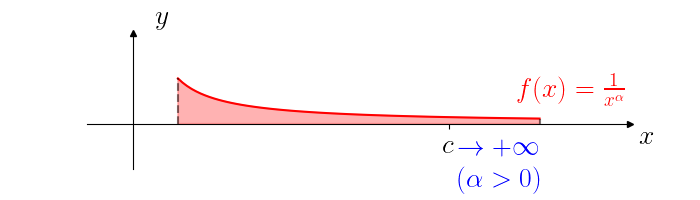
\includegraphics[width=\linewidth]{integrali_impropri/pag77}
		\label{fig:pag77}
	\end{center}

	Fissato $c > 1$, riesco a definire $\int_{1}^{c} f(x)dx$ perché integro una funzione limitata su un intervallo limitato. Posso dunque definire
	\begin{align*}
		\int_{1}^{+\infty} f(x) \ \mathrm{d}x 
		&= \lim_{c\rightarrow +\infty} \int_{1}^{c}f(x) \ \mathrm{d}x \qquad \text{se esiste}
		\\
		\int_{1}^{+\infty} \frac{1}{x^\alpha} dx 
		&= \lim_{c \rightarrow + \infty} \int_{1}^{c} \frac{1}{x^\alpha} \ \mathrm{d} x 
		\\
		&=
		\begin{cases}
			\lim_{c \rightarrow +\infty}\frac{1}{1-\alpha}[c^{1-\alpha}-1] & \text{se } \alpha \neq 1
			\\[1em]
			\lim_{c \rightarrow +\infty} \ln c & \text{se } \alpha=1
		\end{cases}
		\\
		&=
		\begin{cases}
			 \frac{1}{\alpha-1} & \text{se } \alpha > 1
			\\[1em]
			+\infty & \text{se } \alpha \leq 1
		\end{cases}
	\end{align*}
\end{example}
\end{exbar}

	
\begin{exbar}
\begin{example}
	\begin{equation*}
		f(x)=-\ln x, \qquad x \in ]0,1]
	\end{equation*}
	
	e provo a definire 
	\begin{equation*}
		\int_{0}^{1} f(x) \ \mathrm{d}x
	\end{equation*}
	
	cioè l'integrale di una funzione illimitata $\left( \lim_{x \rightarrow 0^+} f(x) = + \infty \right)$ su un intervallo limitato.
	\begin{center}
		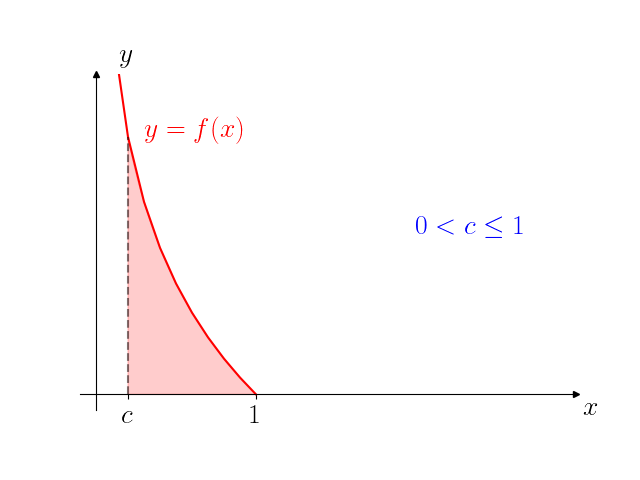
\includegraphics[width=0.75\linewidth]{integrali_impropri/pag79}
		\label{fig:pag79}
	\end{center}
	
	Riesco a definire bene $\int_{c}^{1} f(x) \ \mathrm{d}x$ perché integro una funzione limitata
	$\left( |f(x)|\leq -\ln c \quad \forall \ x \in [c,1] \right)$ su un intervallo limitato.
	
	Posso dunque definire
	\begin{align*}
		\int_{0}^{1} f(x)dx 
		&= \lim_{c\rightarrow +0^+} \int_{c}^{1} f(x) \ \mathrm{d}x \qquad \text{se esiste}
		\\
		\int_{0}^{1}(-\ln x) \ \mathrm{d}x 
		&= \lim_{c \rightarrow 0^+} \int_{c}^{1} (-\ln x) \ \mathrm{d} x
		\\
		&= \lim_{c \rightarrow 0^+} [x-x\ln x]_{c}^{1} 
		\\
		&= \lim_{c \rightarrow 0^+} [1-c+c\ln c]=1
	\end{align*}
\end{example}
\end{exbar}

\begin{definition}
	Sia $f:[a,b[ \ \rightarrow \mathbb{R}; b \in \mathbb{R} \cup\{+\infty\}$ (voglio definire $\int_{a}^{b}f(x) \ \mathrm{d}x$) Riemann integrabile in $[a,c] \ \forall c \in [a,b[$. Se $\exists$ finito il $\lim_{c \rightarrow b^-} \int_{a}^{c} f(x) \ \mathrm{d}x $, allora $f$ si dice integrale in senso improprio o generalizzato in $[a,b[$ e la quantità 
	\begin{equation*}
		\int_{a}^{b} f(x) \ \mathrm{d} x = \lim_{c\rightarrow b^-} \int_{a}^{c} f(x) \ \mathrm{d} x
	\end{equation*}
	si dice integrale improprio o generalizzato di $f$ in $[a,b[$.
	
	Analogamente, data $f:]a,b]\rightarrow \mathbb{R}; a \in \mathbb{R} \cup \{-\infty\}$, Riemann integrabile in $[c,b] \ \forall c \in ]a,b]$. Se $\exists$ finito il $\lim_{c \rightarrow a^+} \int_{c}^{b} f(x) \ \mathrm{d}x$, allora $f$ si dice integrabile in senso improprio o generalizzato in $]a,b]$ e la quantità
	\begin{equation*}
		\int_{a}^{b} f(x) \ \mathrm{d}x = \lim_{c \rightarrow a^+} \int_{c}^{b} f(x) \ \mathrm{d}x
	\end{equation*}
	si dice integrale improprio o generalizzato di $f$ in $]a,b]$.
	
	Se $f$ è integrabile in senso improprio in un intervallo $I$, allora si dice anche che l'integrale (improprio) di $f$ in $I$ è convergente o che $f$ ha integrale (improprio) convergente in $I$.
	
	Se il limite che definisce l'integrale improprio di $f$ è infinito, si dice anche che l'integrale (improprio) di $f$ è divergente o che $f$ ha integrale (improprio) divergente in $I$.
\end{definition}

\begin{attbar}
		Vista la definizione, 
	\begin{equation*}
		\int_{1}^{+\infty} \frac{1}{x^\alpha} \ \mathrm{d}x \text{ converge} \iff \alpha > 1
	\end{equation*}
\end{attbar}

\begin{exbar}
\begin{example} \textbf{importante}
	\begin{align*}
		f(x)=\frac{1}{(x-a)^\alpha}, \qquad
		& x \in ]a, a+1], 
		\\ & a \in \mathbb{R} \text{ fissato}
		\\ & \alpha \in \mathbb{R} \text{ parametro}
		\\ & \alpha > 0
	\end{align*}
	
	Studiamo la convergenza di 
	\begin{align*}
		\int_{a}^{a+1} \frac{1}{(x-a)^\alpha} \ \mathrm{d}x  
		&= \lim_{c \rightarrow a^+} \int_{c}^{a+1} \frac{1}{(x-a)^\alpha} \ \mathrm{d}x
		\\
		&=
		\begin{cases}
			\lim_{c \rightarrow a^+} \frac{1}{1-\alpha} \left[1 - (c-a)^{1-\alpha} \right] & \text{se } \alpha \neq 1 
			\\[1em]
			\lim_{c \rightarrow a^+} -\ln(c-a) & \text{se } \alpha =1
		\end{cases}\\
		&=
		\begin{cases}
			\frac{1}{1-\alpha} & \text{se } \alpha <1 
			\\[1em]
			+\infty & \text{se } \alpha \geq1.
		\end{cases}
	\end{align*}
\end{example}
\end{exbar}

\begin{attbar}
	\begin{equation*}
		\int_{a}^{a+1} \frac{1}{(x-a)^\alpha} \ \mathrm{d}x \text{ converge} \iff \alpha < 1
	\end{equation*}
	
	In particolare
	\begin{equation*}
		\int_{0}^{1} \frac{1}{x^\alpha} \mathrm{d}x \text{ converge} \iff \alpha < 1
	\end{equation*}
\end{attbar}

\begin{exbar}
\begin{example}
	Stabilire se converge 
	\begin{equation*}
		\label{eq:pag 83}
		\int_{0}^{1} \frac{\sin{\frac{1}{x}}}{x^2} \ \mathrm{d}x
	\end{equation*}
	
	\begin{center}
		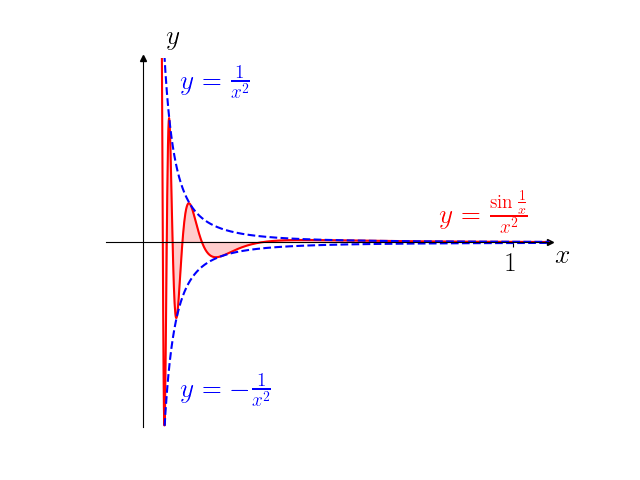
\includegraphics[width=0.75\linewidth]{integrali_impropri/pag83}
		\label{fig:pag83}
	\end{center}
	
		Devo calcolare 
	\begin{equation*}
		\lim_{c\rightarrow0^+} \int_{c}^{1} \frac{\sin{\frac{1}{x}}}{x^2} \ \mathrm{d}x= \lim_{c \rightarrow 0^+} \cos{\frac{1}{x}} \bigg|_{c}^{1}=\lim_{c\rightarrow 0^+}\left(1-\cos{\frac{1}{c}}\right)
	\end{equation*}
	
	che non esiste $\Rightarrow$ la funzione $f(x)=\frac{\sin{\frac{1}{x}}}{x^2}$, non è integrabile in senso improprio in $]0,1]$	
\end{example}
\end{exbar}

\begin{exbar}
\begin{example} \textbf{importante}
	\begin{align*}
		\int_{0}^{+\infty} e^{\alpha x} \ \mathrm{d}x 
		&= \lim_{c \rightarrow +\infty} \int_{0}^{c} e^{\alpha x} \ \mathrm{d}x 
		\\ & =^{\myarrow[10] \alpha \neq 0} \lim_{c \rightarrow +\infty} \frac{1}{\alpha} \ (e^{\alpha c}-1)
		\\
		&= \begin{cases}
			-\frac{1}{\alpha} & \text{se } \alpha <0
			\\
			+\infty & \text{se } \alpha >0.
		\end{cases}
	\end{align*}
\end{example}
\end{exbar}

\begin{attbar}
	\begin{equation*}
		\int_{0}^{+\infty} e^{\alpha x} \ \mathrm{d}x \text{ converge } \iff \alpha < 0
	\end{equation*}
	
	Analogamente
	\begin{equation*}
		\int_{-\infty}^{0} e^{\alpha x} \ \mathrm{d}x \text{ converge } \iff  \alpha > 0
	\end{equation*}
\end{attbar}

Dato $ a>0$, scrivendo $e^{\alpha x} = e^{(\alpha \ln a)x}$ si studia la convergenza degli integrali
\begin{equation*}
	\int_{-\infty}^{0} e^{\alpha x} \ \mathrm{d}x \qquad \int_{0}^{+\infty}  e^{\alpha x} \ \mathrm{d}x.
\end{equation*}

(Utile esercizio per casa)


\textbf{Nota Bene}

$f:[1,+\infty[ \ \rightarrow \mathbb{R}$ continua. E' vero o falso che $\lim_{x \rightarrow +\infty} f(x)=0 \Rightarrow \int_{1}^{+\infty} f(x) \ \mathrm{d}x$ converge?

\begin{center}
	\textbf{È falso!!!} Si veda $f(x)=\frac{1}{x}$
\end{center}

E' vero o falso che
$\int_{1}^{+\infty}f(x) \ \mathrm{d}x$ converge $\Rightarrow \lim_{x \rightarrow +\infty} f(x) = 0$?

\begin{center}
	\textbf{È falso!!!}
\end{center}

\begin{center}
	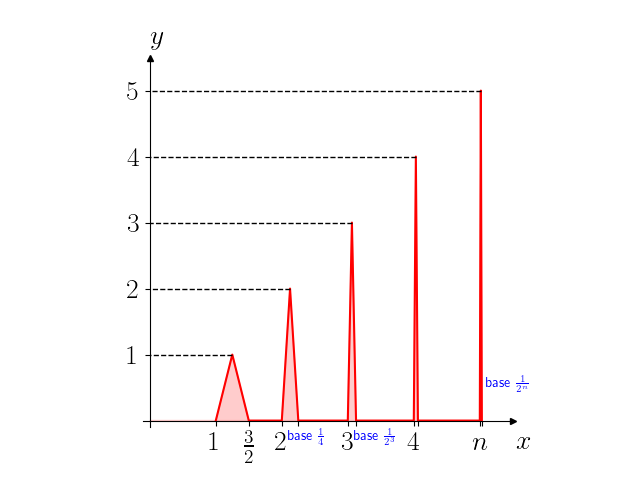
\includegraphics[width=0.75\linewidth]{integrali_impropri/pag85}
	\label{fig:pag85}
\end{center}

Ad ogni numero naturale $n$ costruite un triangolo di base $\frac{1}{2^n}$ e altezza $n$
\begin{equation*}
	\int_{1}^{+\infty} f(x) \ \mathrm{d}x = \sum (\text{aree dei triangoli}) = \sum_{n=1}^{\infty} \frac{1}{2} \frac{1}{2^n} \cdot n = \frac{1}{2} \sum_{n=1}^{\infty} \frac{n}{2^n}, 
\end{equation*}

che è una serie convergente.


\begin{attbar}
	Se $f:[a,b] \rightarrow \mathbb{R}$ è Riemann integrabile, allora è integrabile anche in senso improprio e i due integrali coincidono.
\end{attbar}


\begin{definition}
	$f:[a,b] \ \rightarrow \mathbb{R}, \; a,b \in \mathbb{R} \cup \{\pm \infty\}$, Riemann integrabile in $[c,d] \ \forall \ a < c < d < b$. $f$ si dice integrabile in senso improprio in $ ]a,b[$ se, fissato $\xi \in \ ]a,b[$, lo è in $]a, \xi]$ e in $[\xi,b[$ $\bigg($esistono finiti $\lim_{c \rightarrow a^+} \int_{c}^{\xi} f(x) \ \mathrm{d}x$ e $\lim_{d \rightarrow b^-} \int_{\xi}^{d} f(x) \ \mathrm{d}x \bigg)$ e in tal caso si pone 
	\begin{equation*}
		\int_{a}^{b} f(x)dx = \int_{a}^{\xi} f(x)dx + \int_{\xi}^{b} f(x) dx
	\end{equation*}
	
	Si verifica che la definizione non dipende da punto $\xi$ fissato.
\end{definition}


\begin{exbar}
\begin{example}
	Come si integra $\int_{-\infty}^{+\infty} \frac{1}{1+x^2} \ \mathrm{d}x$?
	
	$x \mapsto \frac{1}{1+x^2}$ è integrabile secondo Riemann in $[c,d] \ \forall  \ c < d$. 
	
	Sia $\xi = 2$. Dobbiamo verificare se la funzione è integrabile in senso improprio in $]-\infty,2] $ e in $ [2, +\infty[$
	\begin{gather*}
		\int_{-\infty}^{2} \frac{1}{1+x^2} \ \mathrm{d}x = \lim_{c \rightarrow -\infty} \int_{c}^{2} \frac{1}{1+x^2} \ \mathrm{d}x = \lim_{c \rightarrow -\infty} \left( \arctan{2 + \frac{\pi}{2}} \right)= \arctan{2 + \frac{\pi}{2}}
		\\
		\int_{2}^{+\infty} \frac{1}{1 + x^2} \ \mathrm{d}x = \lim_{c \rightarrow +\infty} \int_{2}^{c} \frac{1}{1 + x^2} \mathrm{d}x = \lim_{c \rightarrow +\infty} (\arctan{c} - \arctan{2}) = \frac{\pi}{2} - \arctan{2}
		\\
		\Rightarrow \int_{-\infty}^{+\infty} \frac{1}{1+x^2} \ \mathrm{d}x \text{ converge e } \int_{-\infty}^{+\infty} \frac{1}{1+x^2} \ \mathrm{d}x = \int_{-\infty}^{2} \frac{1}{1+x^2} \ \mathrm{d}x + \int_{2}^{+\infty} \frac{1}{1+x^2} \ \mathrm{d}x
	\end{gather*}
\end{example}
\end{exbar}


\begin{exbar}
\begin{example}
	\begin{gather*}
		f(x)=\frac{1}{x^\alpha}, \qquad x \in \ ]0,+\infty[
		\\
		\alpha > 0 \Rightarrow \lim_{x \rightarrow 0^+} f(x)=+\infty.
	\end{gather*}
	
	Preso $\xi=1$, $f$ è integrabile in senso improprio in $]0,+\infty[ \ \iff$ entrambi gli integrali $\int_{0}^{1} \frac{1}{x^\alpha} \ \mathrm{d}x$ e $\int_{1}^{+\infty} \frac{1}{x^\alpha} \ \mathrm{d}x$ convergono. Ma
	\begin{gather*}
		\int_{0}^{1} \frac{1}{x^\alpha} \ \mathrm{d}x \text{ converge} \iff \alpha < 1 
		\\
		\int_{1}^{+\infty} \frac{1}{x^\alpha} \ \mathrm{d}x \text{ converge} \iff \alpha > 1
		\\
		\Rightarrow \int_{0}^{+\infty} \frac{1}{x^\alpha} \ \mathrm{d}x \text{ non converge per alcun valore di } \alpha
	\end{gather*}
\end{example}
\end{exbar}


\begin{exbar}
\begin{example}
	\begin{equation*}
		f(x)= 
		\begin{cases}
			e^x & \text{se } x \leq 1 
			\\
			\frac{1}{x \sqrt{x-1}} & \text{se } x>1
		\end{cases}
	\end{equation*}
	
	vogliamo stabilire se $\int_{-\infty}^{+\infty} f(x) \ \mathrm{d}x$ converge.
	\begin{center}
		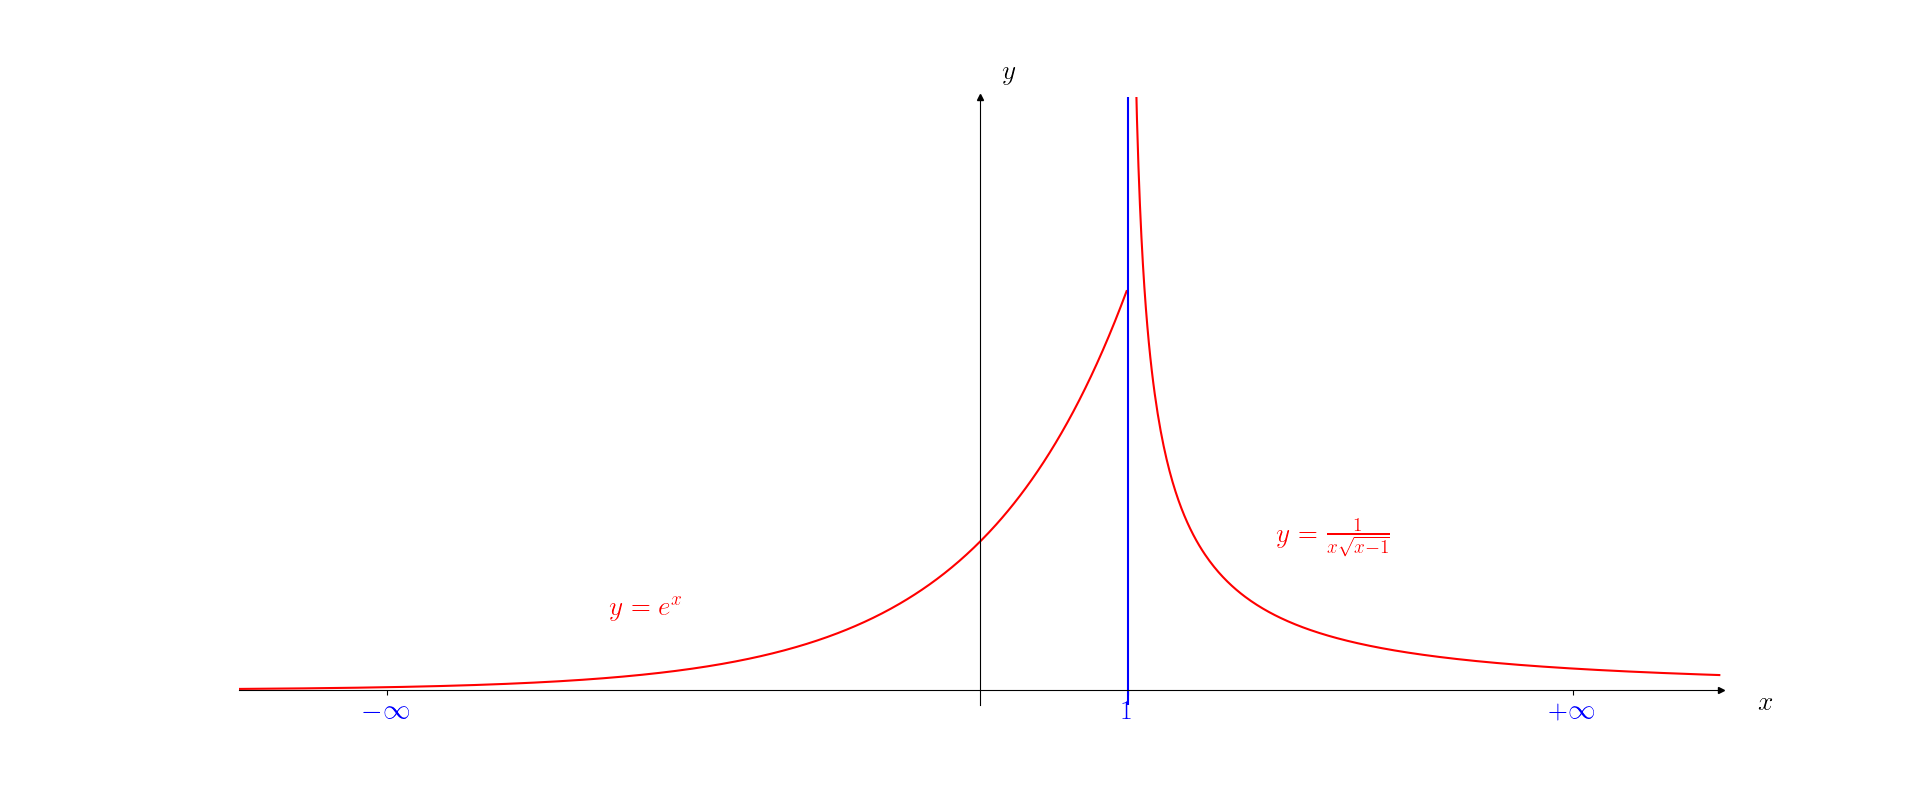
\includegraphics[width=0.75\linewidth]{integrali_impropri/pag89}
		\label{fig:pag89}
	\end{center}
	
	Devo studiare $\int_{-\infty}^{1} f(x) \ \mathrm{d}x = \int_{-\infty}^{1} e^x \ \mathrm{d}x$ e, prendendo $\xi=3$,  $\int_{1}^{3} f(x) \ \mathrm{d}x$ e $\int_{3}^{+\infty} f(x) \ \mathrm{d}x$. Se tutti convergono, anche $\int_{-\infty}^{+\infty} f(x) \ \mathrm{d}x$ converge e 
	\begin{equation*}
		\int_{-\infty}^{+\infty} f(x) \ \mathrm{d}x = \int_{-\infty}^{1} f(x) \ \mathrm{d}x + \int_{1}^{3} f(x) \ \mathrm{d}x + \int_{3}^{+\infty} f(x) \ \mathrm{d}x
	\end{equation*}
\end{example}
\end{exbar}

In generale, data $f:]a,b[ \ \rightarrow \mathbb{R}$ integrabile in senso improprio in $]x_0,x_1[, \ ]x_1,x_2[, \ \ldots, \ ]x_{n-1}, \ x_n[$ con $a = x_0 < x_1 < \ldots < x_n = b$, allora $f$ si dice integrabile in senso improprio in $]a,b[$ e si pone 
\begin{equation*}
	\int_{a}^{b} f(x) \ \mathrm{d}x= \sum_{i=1}^{n} \int_{x_{i-1}}^{x_i} f(x) \ \mathrm{d}x.
\end{equation*}

\subsection{Criteri di integrabilità}
\begin{proposition}
	\label{pr: integrabilità definita}
	Sia $f:[a,b[ \ \rightarrow \mathbb{R}, \ b \in \mathbb{R} \cup \{+\infty\}$ tale che $f(x) \geq 0$ definitivamente per $x \rightarrow b^-$ e tale che sia Riemann integrabile in $[a,b] \ \forall c \in [a,b[$. Allora esiste
	\begin{equation*}
		\lim_{c \rightarrow b^-} \int_{a}^{c} f(x) \ \mathrm{d}x
 	\end{equation*}
	cioè l'integrale improprio $\int_{a}^{b} f(x) \ \mathrm{d}x$ è ben definito (converge o diverge a $+\infty$).
\end{proposition}

\begin{dembar}
	\textbf{Dimostrazione} della \textbf{Proposizione \ref{pr: integrabilità definita}}
	
	
	Per semplicità assumiamo $f(x) \geq 0 \ \forall \ x \in [a,b[$. Sia allora $F(c)=\int_{a}^{c} f(x) \ \mathrm{d}x, \ c \in [a,b[$. 
	
	Allora $F$ è monotona crescente, dunque, presi $c_2 > c_1$ si ha
	\begin{equation*}
		F(c_2) - F(c_1) = \int_{a}^{c_2} f(x) \ \mathrm{d}x - \int_{a}^{c_1} f(x) \ \mathrm{d}x = \int_{c_1}^{c_2} f(x) \ \mathrm{d}x \geq 0
	\end{equation*}
	
	perché $f(x) \geq 0 \ \forall x \in [c_1,c_2] \Rightarrow F(c_2) \geq F_{c_1}$.
	
	$F$ ha limite per $c \rightarrow b^-$, cioè esiste
	\begin{equation*}
		\lim_{c \rightarrow b^-} F(c) = \lim_{c \rightarrow b^-} \int_{a}^{b} f(x) \ \mathrm{d}x.
	\end{equation*}
	
	Un risultato analogo si enuncia per funzioni definitivamente $\leq 0$ per $ x \rightarrow b^-$ o per una funzione $f: \ ]a,b] \rightarrow \mathbb{R}, \ a \in \mathbb{R} \cup \{-\infty\}. \ \square$ 
\end{dembar}


Come per le serie ci concentriamo su criteri di integrabilità per funzioni di segno definito.

\subsubsection{Criterio del confronto}
\begin{theorem} (criterio del confronto)
	
\end{theorem}
	\label{th:criterio del confronto integrale}
	$f,g : [a,b[ \ \rightarrow \mathbb{R}, \ b \in \mathbb{R} \cup \{+\infty\}$, Riemann integrabili in $[a,c] \ \forall c \in [a,b[$ e tali che $0 \leq f(x) \leq g(x)$ definitivamente per $x \rightarrow b^-$.
	\begin{enumerate}
		\item Se $\int_{a}^{b} g(x) \ \mathrm{d}x$ converge, allora converge anche $\int_{a}^{b} f(x) \ \mathrm{d}x$.
		\item Se $\int_{a}^{b} f(x) \ \mathrm{d}x$ diverge, allora diverge anche $\int_{a}^{b} g(x) \ \mathrm{d}x$.
	\end{enumerate}
	Un risultato analogo vale per funzioni $f,g: \ ]a,b] \rightarrow \mathbb{R}, \ a \in \mathbb{R} \cup \{-\infty\}$, con ovvie modifiche.


\begin{dembar}
		\textbf{Dimostrazione} del \textbf{Teorema \ref{th:criterio del confronto integrale}}
		
		Per semplicità assumiamo $0 \leq f(x) \leq g(x) \ \forall \ x \in [a,b[$.
		\begin{enumerate}
			\item $\exists$ finito $\lim_{c \rightarrow b^-} \int_{a}^{c} g(x) \ \mathrm{d}x \ \forall \ c \in [a,b[, \ \int_{a}^{c} f(x) \ \mathrm{d}x \leq \int_{a}^{c} g(x) \ \mathrm{d}x$ perché $f(x) \leq g(x)$. Allora 
			\begin{equation*}
				\undercomment{\lim_{c \rightarrow b^-} \int_{a}^{c} f(x) \ \mathrm{d}x} {\text{esiste perché}} {f(x) \geq 0} \leq \lim_{c \rightarrow b^-} \int_{a}^{c} g(x) \ \mathrm{d}x
			\end{equation*}
			
			e quindi $\lim_{c \rightarrow b^-} \int_{a}^{c} f(x) \ \mathrm{d}x $ esiste finito e $\int_{a}^{b} f(x) \ \mathrm{d}x$ è convergente.
			
			\item $\lim_{c \rightarrow b^-} \int_{a}^{c} f(x) \ \mathrm{d}x = +\infty $ ($f(x)\geq 0$)
			\begin{gather*}
				\int_{a}^{c} g(x) \ \mathrm{d}x \geq \uppercomment{\int_{a}^{c} f(x) \ \mathrm{d}x} {\rightarrow +\infty} {\text{per } c \rightarrow + \infty} \ \forall \ c \in [a,b[
				\\
				\Rightarrow \lim_{c \rightarrow b^-} \int_{a}^{c} g(x) \ \mathrm{d}x = +\infty
			\end{gather*}
			 
			per il teorema del confronto sui limiti. $\square$
		\end{enumerate}
\end{dembar}


\subsubsection{Criterio di assoluta integrabilità}
\begin{theorem}
	\label{th:criterio assoluta integrabilità}
	$f:[a,b[ \ \rightarrow \mathbb{R}, \ b \in \mathbb{R} \cup \{+\infty\}$ Riemann integrabile in $[a,c] \ \forall \ c \in [a,b[$ e tale che $|f|$ è integrabile in senso improprio in $[a,b[$ (si dice che l'integrale improprio di $f$ è assolutamente convergente o che converge assolutamente). Allora $\int_{a}^{b} f(x) \ \mathrm{d}x$ converge.
\end{theorem}


\begin{dembar}
	\textbf{Dimostrazione} del \textbf{Teorema \ref{th:criterio assoluta integrabilità}}
	
	\begin{gather*}
		f = f^+ - f^-
		\\
		f^+ = \max \{f(x), 0\} \geq 0 \quad f^- =\min \{f(x), 0\} \geq 0 \quad \forall \ x
		\\
		\left| f(x) \right| = f^+(x) + f^-(x)
	\end{gather*}
	\begin{center}
		\includegraphics[width=0.75\linewidth]{integrali_impropri/pag94(2)}
		\label{fig:pag94}
	\end{center}

	$f^+$ e $f^-$ sono Riemann integrabili  in  $[a,c] \ \forall \ c \in [a,b[$ e inoltre
	\begin{equation*}
		\begin{array}{c}
			0 \leq f^+(x) \leq |f(x)|
			\\
			0 \leq f^-(x) \leq |f(x)|
		\end{array}
		\qquad \forall \ x \in [a,b[
	\end{equation*}
	$\Rightarrow$ per il criterio del confronto $\int_{a}^{b} f^+(x) \ \mathrm{d}x$ e $\int_{a}^{b} f^-(x) \ \mathrm{d}x$ convergono entrambi 
	\begin{equation*}
		\Rightarrow \lim_{c \rightarrow b^-} \int_{a}^{c} f(x) \ \mathrm{d}x = \lim_{c \rightarrow b^-} \left[ \int_{a}^{c}f^+(x) \ \mathrm{d}x - \int_{a}^{c}f^-(x) \ \mathrm{d}x \right]
	\end{equation*}
	esiste finito per il teorema sulla somma dei limiti $\Rightarrow \int_{a}^{b} f(x) \ \mathrm{d}x$ converge. $\square$
\end{dembar}


\begin{attbar}
	Sia $f: [a,b[ \rightarrow \mathbb{R}, \ b \in \mathbb{R} \cup \{+\infty\}$ e se $\int_{a}^{b} f(x) \ \mathrm{d}x$ converge, non è detto che $\int_{a}^{b} |f(x)| \ \mathrm{d}x$ converga.
\end{attbar}


\begin{exbar}
\begin{example}
	\begin{equation*}
		f(x) = \frac{\sin x}{x}, \qquad x \geq 1
	\end{equation*}
	
	e dimostriamo che $ \int_{1}^{+\infty} \frac{\sin x}{x} \ \mathrm{d}x$ converge. Fissiamo $c>1$
	\begin{gather*}
		\int_{1}^{c} \frac{\sin x}{x} \ \mathrm{d}x= -\frac{\cos x}{x} \bigg|_{1}^{c} - \int_{1}^{c} \frac{\cos x}{x^2} \ \mathrm{d}x = \cos 1 - \frac{\cos c}{c} - \int_{1}^{c} \frac{\cos x}{x^2} \ \mathrm{d}x
		\\
		\lim_{c \rightarrow +\infty} \int_{1}^{c} \frac{\sin x}{x} \ \mathrm{d}x = \lim_{c \rightarrow +\infty} \left[\cos 1 - \uppercomment{\frac{\cos c}{c}} {\myarrow[10] 0} {} - \lowercomment{\int_{1}^{c} \frac{cosx}{x^2} \ \mathrm{d}x} {\lim_{c \rightarrow + \infty} \int_{1}^{c} \frac{\cos x}{x^2} \ \mathrm{d}x} {\text{esiste finito}}\right] 
	\end{gather*}

	
	$\frac{|\cos x|}{x^2} \leq \frac{1}{x^2} \ \forall \ x \geq 1$ e $ \int_{1}^{+\infty} \frac{1}{x^2} \ \mathrm{d}x$ converge 
	
	$\Rightarrow \int_{1}^{+\infty} \frac{|\cos x|}{x^2} \ \mathrm{d}x$ converge per il criterio del confronto 
	
	$\Rightarrow \int_{1}^{+\infty} \frac{\cos x}{x^2} \ \mathrm{d}x$ converge per il criterio di assoluta integrabilità
	
	$\Rightarrow \lim_{c \rightarrow +\infty} \int_{1}^{c} \frac{\sin x}{x} \ \mathrm{d}x = \cos 1 - \int_{1}^{+\infty} \frac{\cos x}{x^2} \ \mathrm{d}x$ esiste finito e dunque $\int_{1}^{+\infty} \frac{\sin x}{x} \ \mathrm{d}x$ converge 
	\\[1em]

	Ma $\int_{1}^{+\infty} |\frac{\sin x}{x}|dx =+\infty$.
	
	Presi $k \geq 1, \ k \in \mathbb{N}$
	\begin{gather*}
		k\pi \leq x \leq (k+1)\pi
		\\
		\frac{1}{(k+1)\pi} \leq \frac{1}{x} \leq \frac{1}{k\pi}
		\\
		\int_{k\pi}^{(k+1)\pi} \frac{(\sin x)}{x} \ \mathrm{d}x \geq \int_{k\pi}^{(k+1)\pi} \frac{1}{(k+1)\pi} (\sin x) \ \mathrm{d}x = \frac{2}{(k+1)\pi} 
		\\
		\int_{1}^{+\infty} \frac{|\sin{x}|}{x} \ \mathrm{d}x \geq \sum_{k=1}^{\infty} \int_{k\pi}^{(k+1)\pi} \frac{|\sin{x}|}{x} \ \mathrm{d}x \geq \sum_{k=1}^{\infty} \frac{2}{(k+1)\pi}=+\infty
	\end{gather*}
	
	perché $\frac{2}{(k+1)\pi} \sim \frac{1}{k}$.
\end{example}
\end{exbar}


\subsubsection{Criterio asintotico del confronto}
\begin{theorem}
	\label{th:criterio asintotico confronto integrale}
	$f,g: [a,b[\rightarrow \mathbb{R}, \ b \in \mathbb{R} \cup \{+\infty\}$, Riemann integrabili in $[a,c] \ \forall c \in [a,b[$ tali che $f(x),g(x)\geq 0$ definitivamente per $x \rightarrow b^-$ e $\lim_{x \rightarrow b^-} \frac{f(x)}{g(x)}= \ell \in [0,+\infty[$
	\begin{enumerate}
		\item Se $\ell \in \ ]0,+\infty[$, allora $ \int_{a}^{b} f(x) \ \mathrm{d}x$ converge $\iff \int_{a}^{b} g(x) \ \mathrm{d}x$ converge.
		
		\item Se $\ell=0$ e $\int_{a}^{b} g(x) \ \mathrm{d}x $ converge, allora $\int_{a}^{b} f(x) \ \mathrm{d}x$ converge.
		
		\item Se $\ell=+\infty$ e $\int_{a}^{b} g(x) \ \mathrm{d}x$ diverge, allora $\int_{a}^{b} f(x) \ \mathrm{d}x$ diverge.
	\end{enumerate}
\end{theorem}


\begin{dembar}
\textbf{Dimostrazione} del \textbf{Teorema \ref{th:criterio asintotico confronto integrale}}
\begin{enumerate}
	\item $\lim_{x \rightarrow b^-} \frac{f(x)}{g(x)} = \ell \in \ ]0,+\infty[$ 
	allora $\frac{\ell}{2} \leq \frac{f(x)}{g(x)} \leq 2\ell$ definitivamente per $x \rightarrow b^-$ perché $]\frac{\ell}{2},2\ell[$ è un intorno di $\ell$. 
	\begin{equation*}
	\begin{array}{c c}
		f(x) \leq 2 \ell g(x) & \text{definitivamente}
		\\
		g(x) \leq \frac{2}{\ell} f(x) & \text{per } x \rightarrow b^-
	\end{array} 
	\end{equation*}
	 
	Se $\int_{a}^{b} g(x) \ \mathrm{d}x$ converge $\Rightarrow \int_{a}^{b} f(x) \ \mathrm{d}x$ converge;
	
	se $\int_{a}^{b} f(x) \ \mathrm{
	d}x$ converge $\Rightarrow \int_{a}^{b} g(x) \ \mathrm{d}x$ converge per il criterio del confronto.
	
	\item $\lim_{x \rightarrow b^-} \frac{f(x)}{g(x)} = 0 \Rightarrow \frac{f(x)}{g(x)} \leq 1 $ definitivamente per $x\rightarrow b^-$ 
	
	$\Rightarrow f(x) \leq g(x)$ definitivamente per $x\rightarrow b^- \Rightarrow $ 
	
	$\Rightarrow$ se $\int_{a}^{b} g(x) \ \mathrm{d}x$ converge, allora $\int_{a}^{b} f(x) \ \mathrm{d}x$ converge per il criterio del confronto.
	
	\item $\lim_{x \rightarrow b^-} \frac{f(x)}{g(x)} = +\infty \Rightarrow \frac{f(x)}{g(x)} \geq 1$ definitivamente per $x \rightarrow b^-$ 
	
	$\Rightarrow f(x) \geq g(x)$ definitivamente per $x \rightarrow b^-$ 
	
	$\Rightarrow$ se $\int_{a}^{b} g(x) \ \mathrm{d}x$ diverge, allora $\int_{a}^{b} f(x) \ \mathrm{d}x$ diverge sempre per il criterio del confronto. $\square$
\end{enumerate}
\end{dembar}


\begin{exbar}
\begin{example} \textbf{importante}
	
	Studiamo la convergenza di 
	\begin{equation*}
		\int_{2}^{+\infty} \frac{1}{x^\alpha (\ln x)^\beta} \ \mathrm{d}x, \qquad \alpha,\beta \in \mathbb{R}
	\end{equation*}
	\begin{itemize}
		\item Se $\alpha > 1 $
		\begin{equation*}
			\int_{2}^{+\infty}\frac{1}{x^\alpha} \ \mathrm{d}x \text{ converge}
		\end{equation*}

		
		\begin{itemize}
			\item Se $\beta \geq 0 $
			\begin{gather*}
				\frac{1}{x^\alpha (\ln x)^\beta} \leq \frac{1}{x^\alpha} \text{ per } x > a
				\\
				\Rightarrow \int_{2}^{+\infty} \frac{1}{x^\alpha(\ln x)^\beta} \ \mathrm{d}x \text{ converge}
			\end{gather*}
			
			\item Se $\beta < 0 $
			\begin{equation*}
				\frac{1}{x^\alpha(\ln x)^\beta} = \frac{(\ln x)^{-\beta}}{x^\alpha}
			\end{equation*}
			
			Preso $\epsilon > 0$ si ha $\ln x \leq x^\epsilon$ definitivamente per $x \rightarrow+\infty$ 
			\begin{equation*}
				\frac{(\ln x)^{-\beta}}{x^\alpha} \leq \frac{x^{-\epsilon \beta}}{x^\alpha}=\frac{1}{x^{\alpha+\epsilon\beta}}
			\end{equation*}
			
			definitivamente per $x\rightarrow +\infty$.
			
			Scelgo $\epsilon$ in modo che $\alpha + \epsilon\beta > 1$, cioè $\epsilon < \uppercomment{\frac{1-\alpha}{\beta}} {\ >0}{}$
			\begin{gather*}
				\Rightarrow \int_{2}^{+\infty} \frac{1}{x^{\alpha+\epsilon\beta}} \ \mathrm{d}x \text{ converge}
				\\
				\Rightarrow \int_{2}^{+\infty} \frac{1}{x^\alpha(\ln x)^\beta} \ \mathrm{d}x \text{ converge.}
			\end{gather*}
		\end{itemize}
		
		\item Se $\alpha < 1 $
		\begin{equation*}
			\int_{2}^{+\infty} \frac{1}{x^\alpha} \ \mathrm{d}x \text{ diverge}
		\end{equation*}

		\begin{itemize}
			\item Se $\beta \geq 0 $ 
			\begin{gather*}
				\frac{1}{x^\alpha(\ln x)^\beta }\geq \uppercomment{??} {\text{integrale}} {\text{divergente}} 
				\\
				\frac{1}{x^\alpha(\ln x)^\beta} = \frac{(\ln x)^{-\beta}}{x^\alpha}.
			\end{gather*}

			Fissato $\epsilon>0, \ \ln x \leq x^\epsilon $ definitivamente per $x \rightarrow +\infty$ 
			
			$(\ln x)^{-\beta} \undercomment{\geq} {-\beta < 0} {} x^{-\epsilon\beta}$ definitivamente per $x \rightarrow +\infty$ 
			
			$\frac{1}{x^\alpha (\ln x)^\beta} \geq \frac{x^{-\epsilon\beta}}{x^\alpha} = \frac{1}{x^{\alpha+\epsilon\beta}}$ definitivamente per $x \rightarrow +\infty$.
			
			Scelgo  $\epsilon$ in modo che $ \alpha + \epsilon\beta < 1, \ \epsilon < \frac{1-\alpha}{\beta} $
			
			\begin{gather*}
				\Rightarrow \int_{2}^{+\infty} \frac{1}{x^{\alpha + \epsilon\beta}} \ \mathrm{d}x \text{ diverge}
				\\
				\Rightarrow \int_{2}^{+\infty} \frac{1}{x^\alpha(\ln x)^\beta} \ \mathrm{d}x 
			\end{gather*}
		
			diverge per il criterio del confronto.
			
			\item  Se $\beta \leq 0 $
			\begin{gather*}
				\frac{1}{x^\alpha(\ln x)^\beta} = \frac{(\ln x)^{-\beta}}{x^\alpha} \undercomment{\geq} {\text{se } x > e} {} \frac{1}{x^\alpha}
				\\
				\int_{2}^{+\infty}\frac{1}{x^\alpha} \ \mathrm{d}x \text{ diverge}
				\\
				\Rightarrow \int_{2}^{+\infty} \frac{1}{x^\alpha (\ln x)^\beta} \ \mathrm{d}x
			\end{gather*}
			
			  diverge per il criterio del confronto.
		\end{itemize}
		
		\item Se $\alpha=1$
		\begin{equation*}
			 \int_{2}^{+\infty} \frac{1}{x(\ln x)^\beta} \ \mathrm{d}x
		\end{equation*}
		\begin{itemize}
			\item Se $\beta=0$
			\begin{equation*}
				\Rightarrow \int_{2}^{+\infty} \frac{1}{x} \ \mathrm{d}x =+\infty
			\end{equation*}
			
			\item Se $\beta \neq 0,1$
			\begin{align*}
				\int_{2}^{+\infty} \frac{1}{x(\ln x)^\beta} \ \mathrm{d}x 
				&= \lim_{c \rightarrow +\infty} \int_{2}^{c} (\ln x)^{-\beta} \frac{1}{x} \ \mathrm{d}x = \lim_{c \rightarrow +\infty} \frac{1}{1-\beta} (\ln x)^{1-\beta} \bigg|_{2}^{c} = 
				\\
				&= 
				\begin{cases}
					\frac{(\ln 2)^{1-\beta}}{\beta - 1} & \text{se } \beta > 1
					\\[1em]
					+\infty & \text{se } \beta < 1
				\end{cases}
			\end{align*}
			
			\item Se $\beta = 1$
			\begin{equation*}
			 	\int_{2}^{+\infty} \frac{1}{x \ln x} \ \mathrm{d}x = \lim_{c \rightarrow +\infty} \int_{2}^{c} \frac{1}{x \ln x} \ \mathrm{d}x = \lim_{c\rightarrow +\infty} \ln(\ln x)\bigg|_{2}^{c} = +\infty
			\end{equation*}
		\end{itemize}
	\end{itemize}	
\end{example}
\end{exbar}


\begin{attbar}
\begin{equation*}
		\int_{2}^{+\infty} \frac{1}{x^\alpha(\ln x)^\beta} \ \mathrm{d}x \text{ converge } \iff \alpha > 1 \text{ o } (\alpha=1 \text{ e } \beta >1)
\end{equation*}
\end{attbar}


\begin{exbar}
\begin{example} \textbf{importante}
	
	Studiamo la convergenza di
	\begin{equation*}
		\int_{0}^{\frac{1}{2}} \frac{1}{x^\alpha |\ln x|^\beta} \ \mathrm{d}x, \qquad \alpha,\beta \in \mathbb{R}
	\end{equation*}
	\begin{align*}
		\int_{0}^{\frac{1}{2}} \frac{1}{x^\alpha|\ln x|^\beta} \ \mathrm{d}x 
		&= \lim_{c \rightarrow 0^+} \int_{c}^{\frac{1}{2}} \frac{1}{x^\alpha |\ln x|^\beta} \ \mathrm{d}x =
		\\
		&\undercomment{=} {t = \frac{1}{x}} {} \lim_{c \rightarrow 0^+} \int_{2}^{\frac{1}{c}} \frac{1}{\frac{1}{t^\alpha} \left| \ln{\frac{1}{t}} \right|^\beta} \left( \frac{1}{t^2} \right) \ \mathrm{d}t =
		\\
		&= \lim_{c \rightarrow 0^+} \int_{2}^{\frac{1}{c}} \frac{1}{t^{2-\alpha} (\ln t)^\beta} \ \mathrm{d}t =
		\\
		&\undercomment{=} {d = \frac{1}{c}} {} \lim_{d \rightarrow +\infty} \int_{2}^{d} \frac{1}{t^{2-\alpha} (\ln t)^\beta} \ \mathrm{d}t =\int_{2}^{+\infty} \frac{1}{t^{2-\alpha}(\ln t)^\beta} \ \mathrm{d}t
	\end{align*}
	che converge $\iff 2-\alpha > 1$ oppure ($2-\alpha = 1$ e $\beta>1$) $\iff \alpha <1 $ oppure ($\alpha =1 \text{ e } \beta>1$)
\end{example}
\end{exbar}

\begin{attbar}
\begin{equation*}
	\int_{0}^{\frac{1}{2}} \frac{1}{x^\alpha |\ln x|^\beta} \ \mathrm{d}x \text{ converge } \iff \alpha < 1 \text{ o } (\alpha=1 \text{ e } \beta >1)
\end{equation*}
\end{attbar}


\begin{exbar}
\begin{example}
	
	Studiare la convergenza dell'integrale improprio
	\begin{equation*}
		\int_{-\infty}^{+\infty} e^{-x^{2}} \ \mathrm{d}x \quad (=\sqrt{\pi})
	\end{equation*}
	
	Devo studiare separatamente 
	\begin{equation*}
		\int_{-\infty}^{0} e^{-x^{2}} \ \mathrm{d}x \qquad \text{e} \qquad \int_{0}^{+\infty} e^{-x^{2}} \ \mathrm{d}x 
	\end{equation*}
	
	e vedere se entrambi convergono. 
	
	$x\mapsto e^{-x^{2}} $ è pari e dunque
	\begin{align*}
		\int_{-\infty}^{0} e^{-x^{2}} \ \mathrm{d}x
		&= \lim_{c \rightarrow -\infty} \int_{c}^{0} e^{-x^{2}} \ \mathrm{d}x \lowercomment{=}{t=-x}{}
		\\
		&= \lim_{c \rightarrow -\infty} \int_{0}^{-c} e^{-t^2} \ \mathrm{d}t \uppercomment{=}{d=-c}{}
		\\
		&= \lim_{d\rightarrow +\infty} \int_{0}^{d} e^{-x^{2}} \ \mathrm{d}x = \int_{0}^{+\infty} e^{-x^{2}} \ \mathrm{d}x
	\end{align*}
	\begin{gather*}
		\int_{-\infty}^{0} e^{-x^{2}} \ \mathrm{d}x \text{ converge } \iff \int_{0}^{+\infty} e^{-x^{2}} \ \mathrm{d}x \text{ converge.}
		\\
		0 \leq e^{-x^2} \leq e^{-x} \ \forall x \geq 1 \text{ e } \int_{0}^{+\infty}e^{-x} \ \mathrm{d}x = 1 \text{ cioè converge}
	\end{gather*}
	
	 $\Rightarrow$ per il criterio del confronto $\int_{0}^{+\infty} e^{-x^2}dx$ converge.
\end{example}
\end{exbar}


\begin{exbar}
\begin{example}
		
	Studiare la convergenza dell'integrale improprio 
	\begin{equation*}
		\int_{1}^{+\infty} \frac{x^\alpha e^{x^4}}{1+e^{4x^4}} \ \mathrm{d}x \qquad \text{ al variare di } \alpha \in \mathbb{R}.
	\end{equation*}
	
	Per $x \rightarrow +\infty$
	\begin{gather*}
		\frac{x^\alpha e^{x^4}}{1+e^{4x^4}} \sim \frac{x^\alpha e^{x^4}}{x^{4x^4}} = x^\alpha e^{-3x^4}
		\\
		\int_{1}^{+\infty}\frac{x^\alpha e^{x^4}}{1+e^{4x^4}} \ \mathrm{d}x \text{ converge } \iff \int_{1}^{+\infty} x^\alpha e^{-3x^4} \ \mathrm{d}x \text{ converge}
	\end{gather*}
	
	(Provare per casa ponendo $x=\ln t$).
	
	Sicuramente $x^\alpha \leq e^{x^4}$ definitivamente per $x \rightarrow +\infty$ e dunque $x^\alpha e^{-3x^4} \leq e^{-2x^4}\leq e^{-x} $ per $x \geq 1$
	
	$\Rightarrow \int_{1}^{+\infty} x^\alpha e^{-3x^4}dx $ converge per il criterio del confronto $\forall \ \alpha \in \mathbb{R}$.
\end{example}
\end{exbar}


\begin{exbar}
\begin{example}
	
	
	Studiare la convergenza di 
	\begin{gather*}
		\int_{0}^{\mathcircled{+\infty}} \lowercomment{\frac{\ln(3 + \sin x)}{\sqrt[4]{x^5 - x^3 + 3}}} {\geq 0} {} \ \mathrm{d}x
		\\
		\ln 2 \leq \ln(3 + \sin x) \leq \ln 4 \qquad \forall x 
	\end{gather*}
	
	$\exists \ a \in \mathbb{R} \ \bigg| \ \frac{\ln(3 + \sin x)}{\sqrt[4]{x^5 - x^3 + 3}} $ è illimitata in un intorno di $a$?
	
	$\exists \ a \in \mathbb{R}  \ \bigg| \ \sqrt[4]{x^5-x^3+3} \big|_{x=a}=0$, cioè $\exists \ a \in \mathbb{R} \bigg| x^5 - x^3 + 3 \bigg|_{x=a} = 0$?
	\begin{align*}
		g(x)=x^5 - x^3 + 3 & g(1)=3 > 0
		\\
		g'(x) = 5x^4 - 3x^2 = x^2 (5x^2 - 3) > 0 & \forall x >1
	\end{align*}
	
	$\Rightarrow g$ è strettamente crescente in $[1,+\infty[$
	
	$\Rightarrow g(x) \geq g(1)=3 \qquad \forall x \geq 1$
	\begin{equation*}
		\frac{\ln(3+\sin x)}{\sqrt[4]{x^5 - x^3 + 3}} \leq \frac{\ln 4}{\sqrt[4]{x^5 - x^3 + 3}} \underbracket[0pt][0pt]{\sim}_{\text{ per } x \rightarrow +\infty} \frac{1}{x^{\frac{5}{4}}}
	\end{equation*}
	
	che ha integrale convergente in $[1, +\infty[$ e quindi l'integrale dato converge per il criterio del confronto e per il criterio asintotico del confronto.	
\end{example}
\end{exbar}


\begin{attbar}
	\begin{equation*}
		\frac{1}{x^{\frac{5}{4}}}  \sim \frac{\ln 2}{\sqrt[4]{x^5 - x^3 + 3}} \leq \frac{\ln(3 + \sin x)}{\sqrt[4]{x^5 - x^3 + 3}} \leq  \frac{\ln 4}{\sqrt[4]{x^5 - x^3 + 3}} \sim \frac{1}{x^{\frac{5}{4}}}
	\end{equation*}
	
	Se $\int_{1}^{+\infty} \frac{1}{x^{\frac{5}{4}}} \ \mathrm{d}x$ converge, allora converge $ \int_{1}^{+\infty} \frac{\ln(3 + \sin x)}{\sqrt[4]{x^5 - x^3 + 3}} \ \mathrm{d}x$, ma vale anche che, se converge $\int_{1}^{+\infty} \frac{\ln(3+\sin x)}{\sqrt[4]{x^5 - x^3 + 3}} \ \mathrm{d}x$, allora converge $\int_{1}^{+\infty} \frac{1}{x^{\frac{5}{4}}} \ \mathrm{d}x$.
\end{attbar}


\begin{exbar}
\begin{example}
	Al variare di $\alpha, \ \beta > 0$ studiare la convergenza dell'integrale improprio
	\begin{gather*}
		\int_{0}^{1} \frac{3 + \sin{(e^{\frac{1}{t}})}} {[1 + \cos{(\pi t)}]^\alpha| \ln t |^\beta} \ \mathrm{d}t
		\\
		\lim_{t \rightarrow o^+}  \frac{3 + \sin{(e^{\frac{1}{t}})}} {[1 + \cos{(\pi t)}]^\alpha| \ln t |^\beta} = 0
	\end{gather*}
	
	La funzione integranda è Riemann integrabile in $[0,c] \ \forall \ c \in [0,1[$
	\begin{gather*}
		\lim_{t \rightarrow 1^-}  \frac {\uppercomment{{3 + \sin{(e^{\frac{1}{t}})}}} {\myarrow[10] 2\leq 3 + \sin e^{1/t} \leq 4} {}}
		{[1+\cos{(\pi t)}]^\alpha|\ln t |^\beta} =+\infty
		\\
		\mathcircled{\frac{2}{[1 + \cos{(\pi t)}]^\alpha |\ln t |^\beta}} 
		\leq
		\frac{3 + \sin{(e^{\frac{1}{t}})}} {[1 + \cos{(\pi t)}]^\alpha |\ln t |^\beta} 
		\leq 
		\mathcircled{\frac{4}{[1 + \cos{(\pi t)}]^\alpha |\ln t |^\beta}} 
		\\
		\sim  \frac{1}{[1+\cos{(\pi t)}]^\alpha|\ln t |^\beta} \text{ per } x \rightarrow 1
		\\
		\int_{0}^{1} \frac{3 + \sin{(e^{\frac{1}{t}})}} {[1 + \cos{(\pi t)}]^\alpha |\ln t |^\beta} \ \mathrm{d}t  \text{ converge } \iff  \int_{0}^{1} \frac{1}{[1 + \cos{(\pi t)}]^\alpha |\ln t |^\beta} \ \mathrm{d}t \text{ converge}.
		\\
		\ln (1+y) = y + o(y)  \text{ per } y \rightarrow 0 
		\\
		\ln t = \ln(1 + (t - 1)) = t - 1 + o(t - 1)  \text{ per } t \rightarrow 1 
	\end{gather*}
	\begin{align*}	
		\cos( \pi t) &= \cos(\pi) + \cos'(\pi t)\bigg|_{t=1} + \frac{1}{2} \cos''(\pi t)\bigg|_{t=1} (t-1)^2 + o((t-1)^2)
		\\ 
		& = -1 +\frac{\pi^2}{2} (t - 1)^2 + o((t - 1)^2)
	\end{align*}
	\begin{gather*}
		\left(
		\begin{array}{l}
		\frac{d}{dt} \cos(\pi t) = -\pi \sin(\pi t)
		\\
		\frac{d^2}{dt^2} \cos(\pi t) = -\pi^2 \cos(\pi t)
		\end{array}
		\right)
		\\
		1 + \cos(\pi t)= \frac{\pi^2}{2} (t - 1)^2 + o((t - 1)^2)
		\\
		|\ln t|^\beta = |t - 1|^\beta + o(|t - 1|^\beta)
		\\
		(1 + \cos(\pi t))^\alpha = \left( \frac{\pi^2}{2} \right) ^\alpha |t-1|^{2\alpha} + o((t-1)^{2\alpha}) \text{ per } t \rightarrow 1
		\\
		[1 + \cos(\pi t)]^\alpha |\ln t|^\beta = \left(\frac{\pi^2}{2}\right)^\alpha |t-1|^{2\alpha+\beta} +o(|t-1|^{2\alpha+\beta})
		\\
		\frac{1}{[1 + \cos(\pi t)]^\alpha |\ln t|^\beta} \sim \frac{1}{|t-1|^{2\alpha+\beta}}
		\\ 
		\text{e } \int_{0}^{1} \frac{1}{|t-1|^{2\alpha+\beta}} \ \mathrm{d}t  \text{ converge }  \iff 2 \alpha + \beta < 1
	\end{gather*}
	L'integrale di partenza converge $\iff 2 \alpha +\beta < 1$.
\end{example}
\end{exbar}


\begin{exbar}
\begin{example}
	Al variare di $\alpha \in \mathbb{R} $ studiare la convergenza dell'integrale improprio
	\begin{equation*}
		\int_{\mathcircled{0}}^{\mathcircled{+\infty}} \frac{\sinh{x^2}}{x^\alpha e^{\alpha(x^2+x)}} \ \mathrm{d}x
	\end{equation*}
	
	A priori, la funzione potrebbe essere illimitata in un intorno di $x=0$
	
	Dobbiamo studiare la convergenza degli integrali impropri 
	\begin{equation*}
		\int_{0}^{1} \frac{\sinh{x^2}}{x^\alpha e^{\alpha(x^2 + x)}} \ \mathrm{d}x \text{ e } 
		\int_{1}^{+\infty} \frac{\sinh{x^2}}{x^\alpha e^{\alpha(x^2 + x)}} \ \mathrm{d}x
	\end{equation*}
	
	Studiamo $\int_{0}^{1} \frac{\sinh{x^2}}{x^\alpha e^{\alpha(x^2 + x)}} \ \mathrm{d}x$
	\begin{gather*}
		\sinh{y} = \frac{e^y - e^{-y}}{2} = y + o(y) \text{ per } y \rightarrow 0
		\\
		\frac{\sinh{x^2}}{x^\alpha e^{\alpha(x^2 + x)}} \sim \frac{x^2}{x^\alpha} = \frac{1}{x^{\alpha-2}}  \text{ per } x \rightarrow 0
	\end{gather*}
	
	Poiché $\int_{0}^{1} \frac{1}{x^{\alpha-2}} \ \mathrm{d}x$ converge $\iff \alpha -2 < 1 \iff \alpha < 3$, anche $\int_{0}^{1} \frac{\sinh{x^2}}{x^\alpha e^{\alpha(x^2 + x)}} \ \mathrm{d}x$ converge $\iff \alpha < 3$ per il criterio asintotico del confronto.
	
	Studiamo 
	\begin{gather*}
		\int_{1}^{+\infty} \frac{\sinh{x^2}}{x^\alpha e^{\alpha(x^2 + x)}} \ \mathrm{d}x
		\\
		\frac{\sinh{x^2}}{x^\alpha e^{\alpha(x^2 + x)}} \ \mathrm{d}x \sim \frac{e^{x^2}}{x^\alpha e^{\alpha(x^2 + x)}} = \frac{e^{(1 - \alpha)x^2 - \alpha x}}{x^\alpha}  \text{ per } x \rightarrow +\infty
	\end{gather*}
	
	Per il criterio asintotico del confronto $\int_{1}^{+\infty} \frac{\sinh{x^2}}{x^\alpha e^{\alpha(x^2 + x)}} \ \mathrm{d}x$ converge $\iff \int_{1}^{+\infty}  \frac{e^{(1-\alpha) x^2 - \alpha x}}{x^\alpha} \ \mathrm{d}x$ converge.
	
	\begin{itemize}
		\item Se $1-\alpha > 0, \ \alpha < 1$ si avrà
		\begin{gather*}
			\lim_{x\rightarrow +\infty}   \frac{e^{(1-\alpha)x^2-\alpha x}}{x^\alpha} =+\infty 
			\\
			\Rightarrow \int_{1}^{+\infty}  \frac{e^{(1-\alpha)x^2-\alpha x}}{x^\alpha} \ \mathrm{d}x  \text{ diverge.}
		\end{gather*}
		
		\item Se $ 1 - \alpha \leq 0, \ \alpha \geq 1$
		\begin{itemize}
			\item Per $\alpha = 1$ si ha
			\begin{equation*}
				\frac{e^{-x}}{x}  \text{ e } \int_{1}^{+\infty} \frac{e^{-x}}{x} \ \mathrm{d}x  \text{ converge}
			\end{equation*}
			
			\begin{gather*}
				\int_{1}^{+\infty} x^\beta e^{-x} \ \mathrm{d}x, \qquad \beta \in \mathbb{R}
				\text{ definitivamente per } x\rightarrow +\infty
				\\
				x^{\beta} e^{-x} \leq e^{-\frac{x}{2}} \text{ perché} 
				\\ 
				\lim_{x \rightarrow +\infty} \frac{x^\beta e^{-x}}{e^{-\frac{x}{2}}} = \lim_{x\rightarrow +\infty} x^{\beta} e^{-\frac{x}{2}} = 0
				\\				\int_{1}^{+\infty}e^{-\frac{x}{2}} \ \mathrm{d}x  \text{ converge } \Rightarrow \int_{1}^{+\infty} x^\beta e^{-x} \ \mathrm{d}x
				\end{gather*}
				
				converge per il criterio del confronto.
			\begin{equation*}
				\Rightarrow \int_{1}^{+\infty} \frac{e^{-x}}{x} \ \mathrm{d}x \text{ converge.}
			\end{equation*}
			
			\item Per $-1 - \alpha <0, \qquad \alpha > 1$
			\begin{equation*}
				\frac{e^{(1 - \alpha) x^2 - \alpha x}}{x^\alpha} = \frac{e^{(1 - \alpha) x^2} e^{-\alpha x}}{x^\alpha} \undercomment{\leq} {x\geq1} {} \frac{e^{(1 - \alpha) x^2}}{x^\alpha} \leq e^{-x}
			\end{equation*}
			
			definitivamente per $x \rightarrow +\infty$ perché
			\begin{gather*}
				\lim_{x \rightarrow +\infty} \frac{\frac{e^{(1 - \alpha) x^2}} {x^\alpha}} {e^{-x}} = \lim_{x \rightarrow +\infty} \frac{e^{ (1 - \alpha) x^2 + x}}{x^\alpha} = 0
				\\
				\int_{1}^{+\infty} e^{-x} \ \mathrm{d}x  \text{ converge } \Rightarrow \int_{1}^{+\infty}\frac{e^{(1 - \alpha) x^2}}{x^\alpha} \ \mathrm{d}x  \text{ converge} 
			\end{gather*}
			
			$\Rightarrow$ converge anche l'integrale di partenza
			\begin{equation*}
				\int_{0}^{+\infty} \frac{\sinh{x^2}}{x^\alpha e^{\alpha(x^2+x)}}\ \mathrm{d}x  \text{ converge } \iff 1 \leq \alpha < 3.
			\end{equation*}
		\end{itemize}
	\end{itemize}
\end{example}
\end{exbar}


\begin{exbar}
\begin{example} \textbf{importante}
	
	Sia 
	\begin{equation*}
		\Gamma(x) = \int_{0}^{+\infty} t^{x-1} e^{-t} \ \mathrm{d}t, \qquad x > 0
	\end{equation*}
	
	(funzione gamma di Eulero.)
	\begin{enumerate}
		\item Provare che $\Gamma$ è ben definita e che $\Gamma(x) \in \mathbb{R} \qquad \forall \ x > 0$
		\item Provare che $\Gamma(x+1)=x \ \Gamma(x) \qquad \forall \ x > 0$
	\end{enumerate}
	
	\vspace{2em}
	\begin{enumerate}
		\item $t \mapsto t^{x-1} e^{-t}$ è positiva e quindi l'integrale improprio converge o diverge a $+\infty$.
		
		Dimostriamo che converge $\forall \ x > 0$.
		
		Devono convergere entrambi gli integrali
		\begin{equation*}
			\int_{0}^{1} t^{x-1} e^{-t} \ \mathrm{d}t \text{ e } \int_{1}^{+\infty} t^{x-1} e^{-t} \mathrm{d}t.
		\end{equation*}
		
		Vediamo il primo
		\begin{align*}
			t^{x-1} e^{-t} \sim t^{x-1} &\text{ per } t \rightarrow 0
			\\
			\Rightarrow \int_{0}^{1}t^{x-1} \mathrm{d}t =\int_{0}^{1} \frac{1}{t^{1-x}} \ \mathrm{d}t & \text{ converge} \iff 1 - x < 1 \iff x > 0
		\end{align*}
		
		Per il criterio asintotico del confronto $\int_{0}^{1} t^{x-1} e^{-t} \ \mathrm{d}t$ converge $\iff x > 0$.
		
		Vediamo $\int_{1}^{+\infty} t^{x-1} e^{-t} \ \mathrm{d}t$
		
		Abbiamo già visto che gli integrali di questo tipo convergono $\forall x$ perché $t^{x-1} e^{-t} \leq e^{-\frac{t}{2}}$ definitivamente per $t \rightarrow +\infty$
		
		\begin{equation*}
			\Rightarrow \Gamma(x) = \int_{0}^{+\infty} t^{x-1} e^{-t} \ \mathrm{d}t \text{ converge} \qquad \forall \ x >0
		\end{equation*}
		
		\item $\Gamma(x+1) = x \ \Gamma(x) \qquad \forall \ x > 0$
		\begin{align*}
			\Gamma(x+1)
			&=\int_{0}^{+\infty} t^{x} e^{-t} \ \mathrm{d}t =
			\\
			&=  \lim_{c \rightarrow + \infty} \int_{0}^{c} t^{x} e^{-t} \ \mathrm{d}t =
			\\
			&= \lim_{c \rightarrow + \infty} \left[ -t^x e^{-t} \bigg|_{0}^c + x \int_{0}^{c} t^{x-1} e^{-t} \ \mathrm{d}t \right] = 
			\\
			&= \lim_{c \rightarrow + \infty} \left[ -c^x e^{-c} + \int_{0}^{c} t^{x-1} e^{-t} \ \mathrm{d}t \right] = 
			\\
			&= x \ \Gamma(x)
		\end{align*}
		\begin{equation*}
			\Gamma(1) = \int_{0}^{+\infty} t^{1 - 1} e^{-t} \ \mathrm{d}t = \int_{0}^{+\infty} e^{-t} \ \mathrm{d}t = 1
		\end{equation*}
		
		Per $n \in \mathbb{N}$
		\begin{align*}
			\Gamma(n+1)
			&= n \ \Gamma(n) = n \ \Gamma((n-1)+1) = n (n-1) \ \Gamma(n-1) =
			\\
			&= n(n-1) \ \Gamma((n-2)+1) = n(n-1)(n-2) \ \Gamma(n-2) = \ldots =
			\\
			&= n(n-1)(n-2) \cdot \ldots \cdot 2 \ \Gamma(1) = n(n-1)(n-2)(n-3) \cdot \ldots 2 \cdot 1 = n!    
		\end{align*}
	\end{enumerate}
\end{example}
\end{exbar}


\subsubsection{Integrali oscillanti}
\begin{theorem} (criterio di Abel)
\label{th: criterio di Abel}

Sia  $a \in \mathbb{R}, \quad f,G : [a,+\infty[ \ \rightarrow \mathbb{R}$ di classe $C^1$ tali che
\begin{enumerate}
	\item $f'(x) \leq 0 \qquad \forall \ x \geq a$ e $\lim_{x \rightarrow +\infty} f(x) = 0$
	\item $G$ è limitata, cioè $\exists \ C > 0$ tale che $ |G(x)| \leq C \qquad \forall \ x \geq a$
\end{enumerate}

Allora $\int_{a}^{+\infty} f(x) \ G'(x) \ \mathrm{d}x$ converge.
\end{theorem}


\begin{dembar}
	\textbf{Dimostrazione} del \textbf{Teorema \ref{th: criterio di Abel}}
	
	\begin{align*}
		\int_{a}^{+\infty} f(x) \ G'(x) \ \mathrm{d}x
		&=\lim_{\omega \rightarrow +\infty} \int_{a}^{\omega} f(x) \ G'(x) \ \mathrm{d}x 
		\\
		\int_{a}^{\omega} f(x) \ G'(x) \ \mathrm{d}x
		& \undercomment{=} {\text{integro}} {\text{per parti}} f(x) \ G(x) \bigg|_{a}^{\omega} - \int_{a}^{\omega} f'(x) \ G(x) \ \mathrm{d}x =
		\\
		&= \lowercomment{f(\omega) \ G(\omega)} {\myarrow[350] 0 \text{ perché} f(\omega) \rightarrow 0} {\text{e } G \text{ è limitata}} - f(a) \ G(a) - \int_{a}^{\omega} f'(x) \ G(x) \ \mathrm{d}x =
		\\
		\int_{a}^{+\infty} f(x) \ G'(x) \ \mathrm{d}x
		&= -f(a) \ G(a) - \lim_{\omega \rightarrow +\infty} \int_{a}^{\omega} f'(x) \ G(x) \ \mathrm{d}x
	\end{align*}
	
	Se dimostro che $\lim_{\omega \rightarrow +\infty} \int_{a}^{\omega} f'(x) \ G(x) \ \mathrm{d}x$ esiste finito, cioè che $\int_{a}^{+\infty} f'(x) \ G(x) \ \mathrm{d}x$ è convergente, deduco che converge anche $\int_{a}^{+\infty} f(x) \ G'(x) \ \mathrm{d}x$.
	
	Dimostriamo che l'integrale $\int_{a}^{+\infty} f'(x) \ G(x) \ \mathrm{d}x$ converge assolutamente
	\begin{gather*}
		\int_{a}^{+\infty} \big|f'(x) \ G(x) \big| \ \mathrm{d}x = \underbracket[0pt][0pt]{\lim_{\omega \rightarrow +\infty} \int_{a}^{\omega} \big|f'(x) \ G(x) \big| \ \mathrm{d}x}
		_{\genfrac{}{}{0pt}{}
		{\color{blue}{\text{il limite esiste, devo}}}
		{\color{blue}{\text{far vedere che è finito}}}} \leq C \ f(a) < +\infty
		\\
		\int_{a}^{\omega} \big|f'(x) \ G(x) \big| \ \mathrm{d}x 
		\undercomment{\leq} {\big| G(x) \big| \leq C} {} C \int_{a}^{\omega} \big| f'(x) \big| \ \mathrm{d}x 
		\undercomment{=} {f'(x) \leq 0} {} -C \int_{a}^{\omega} f'(x) \ \mathrm{d}x = C \left[ f(a) - f(\omega) \right] 
		\undercomment{\leq} {f(\omega) \geq 0} {} C f(a) \quad \forall \omega \quad \square
	\end{gather*}
\end{dembar}
	
	
\begin{exbar}
\begin{example}
	\begin{gather*}
		\int_{1}^{+\infty} \frac{\sin x}{x} \ \mathrm{d}x \text{ converge}
		\\
		f(x) = \frac{1}{x} \qquad G(x) = -\cos x
		\\
		\int_{1}^{+\infty} \frac{\sin x}{x} \ \mathrm{d}x = \int_{1}^{+\infty} f(x) \ G'(x) \ \mathrm{d}x
	\end{gather*}
\end{example}
\end{exbar}


\begin{exbar}
\begin{example}
	
	Studiare la convergenza di 
	\begin{equation*}
		\int_{0}^{+\infty} \cos(e^x) dx
	\end{equation*}
	
	(Diverge assolutamente, $ \int_{0}^{+\infty} \big| \cos(e^x) \big| \ \mathrm{d}x = +\infty$)
	\begin{gather*}
		\int_{0}^{+\infty} \cos(e^x) \ \mathrm{d}x = \int_{0}^{+\infty} \underbrace{e^{-x}}_{f(x)} \cdot \underbrace{e^{x} \cos(e^x)}_{G'(x)} \ \mathrm{d}x
		\\
		G(x) = \sin(e^x) \text{ e } \big| G(x) \big| \leq 1 \qquad \forall x 
	\end{gather*}
	
	$\Rightarrow$ l'integrale converge per il criterio di Abel.
	
	\begin{align*}
		\int_{0}^{+\infty} \cos(e^x) \ \mathrm{d}x &= \lim_{c \rightarrow +\infty} \int_{0}^{c} \cos(e^x) \ \mathrm{d}x \undercomment{=} {t=e^x} {} \lim_{c \rightarrow +\infty} \int_{0}^{e^c} \frac{\cos(t)}{t} \ \mathrm{d}t =
		\\
		&= \int_{1}^{+\infty} \frac{\cos(t)}{t} \ \mathrm{d}t \text{ che converge}
	\end{align*}
\end{example}
\end{exbar}


\begin{exbar}
\begin{example}
	
	Studiare la convergenza di 
	\begin{equation*}
		\int_{0}^{+\infty} \cosh x \frac{\sin(\sinh x)}{x^\alpha} \ \mathrm{d}x
	\end{equation*}
	al variare di $\alpha >0$.
	
	Devo studiare la convergenza di 
	\begin{equation*}
		\int_{0}^{2} \cosh x \frac{\sin(\sinh x)}{x^\alpha} \ \mathrm{d}x \text{ e } \int_{2}^{+\infty} \cosh x \frac{\sin(\sinh x)}{x^\alpha} \ \mathrm{d}x
	\end{equation*}
	\begin{itemize}
		\item Vediamo il primo.
		
		$\cosh x\frac{\sin(\sinh x)}{x^\alpha}$ è definitivamente positiva per $x \rightarrow 0$
		
		$ \lowercomment{\cosh x} {1 \text{ per } x \rightarrow 0} {} \frac{ \uppercomment{\sin(\sinh x)} {= \sinh x +o(\sinh x) \text{ perché}} {\sinh x \rightarrow 0 \text{ per } x \rightarrow 0}}{x^\alpha} \sim \frac{\sinh x}{x^\alpha}\sim \frac{x}{x^\alpha}=\frac{1}{x^{\alpha-1}}\sim  \int_{0}^{2} \frac{1}{x^{\alpha-1}} \ \mathrm{d}x$ converge $\iff \alpha-1 < 1 \iff \alpha < 2$
		
		$ \int_{0}^{2} \cosh x \ \frac{\sin(\sinh x)}{x^\alpha} \ \mathrm{d}x$ converge $\iff \alpha < 2$ per il criterio asintotico del confronto.
		

		
		\item Vediamo il secondo.\\
		$\int_{2}^{+\infty} \cosh x\frac{\sin(\sinh x)}{x^\alpha}dx$ con $\alpha >0$,\\ $f(x)=\frac{1}{x^\alpha}$ (decrescente infinitesima),\\
		$G(x)=-\cos(\sinh x)$, cosicchè $G'(x)=\cosh x \sin(\sinh x)$ (limitata $|G(x)|\leq 1$),\\
		$\int_{2}^{+\infty} \cosh x\frac{\sin(\sinh x)}{x^\alpha}dx = \int_{2}^{+\infty} f(x)G'(x)dx$ converge per il criterio di Abel $\Rightarrow \int_{2}^{+\infty} \cosh x\frac{\sin(\sinh x)}{x^\alpha}dx$, se $ \alpha > 0$ converge $\Leftrightarrow \alpha <2$. 
	\end{itemize}
\end{example}
\end{exbar}
	
	
	
\begin{comment}	


\paragraph{\textcolor{red}{Osservazione}}
$f:[0,+\infty[\rightarrow\R$ positiva, decrescente, infinitesima a $+\infty$. Consideriamo
\begin{equation*}
	\int_{0}^{+\infty} f(x)\sin xdx
\end{equation*}
Come studiare la convergenza senza utilizzare il criterio di Abel?\\
\textcolor{orange}{$|f(x)\sin x|\leq f(x)$ se $\int_{0}^{+\infty}f(x)dx$ converge $\Rightarrow \int_{0}^{+\infty}f(x)\sin x dx$ converge assolutamente e quindi converge e se $\int_{0}^{+\infty}f(x)dx$ diverge?}\\
$\sin x \geq 0$ se $ 2k\pi \leq x \leq (2k+1)\pi$ e $\sin x \leq 0$ se $(2k+1)\pi \leq x \leq (2k+1)\pi$
\begin{align*}
	\int_{k\pi}^{(k+1)\pi}f(x)\sin x dx &= (-1)^k\int_{k\pi}^{(k+1)\pi}f(x)|\sin x|dx\\
	\int_{0}^{+\infty}f(x)\sin x dx &=\sum_{k=0}^{\infty} (-1)^k \int_{k\pi}^{(k+1)\pi}f(x)|\sin x|dx=\sum_{k=0}^{\infty} (-1)^k a_k
\end{align*}
$a_k \geq 0 \Rightarrow$
\begin{equation*}
	a_{k+1}= \int_{(k+1)\pi}^{(k+2)\pi}f(x)|\sin x|dx \leq \int_{k\pi}^{(k+1)\pi}f(x)|\sin x|dx=a_k
\end{equation*}
\begin{equation*}
	0\leq a_k = \int_{k\pi}^{(k+1)\pi}f(x)|\sin x|dx \leq \int_{k\pi}^{(k+1)\pi}f(x)dx\leq \pi f(k\pi)\rightarrow 0
\end{equation*}
\textcolor{orange}{$f(x)\leq f(k\pi) \,\,\, \forall x\in [k\pi,(k+1)\pi]$}\\
La serie converge per il criterio di Leibniz.

\subsection{\textcolor{red}{Spazi Metrici e Normati}}
\paragraph{\textcolor{red}{Definizione}}
$X$ spazio vettoriale su $\R$ o $\C$. Una \textcolor{red}{norma} su $X$ è una funzione $\parallel \cdot \parallel : X\rightarrow \R$ tale che 
\begin{enumerate}
	\item $\parallel x\parallel\geq 0 \forall x \in X$ e $\parallel x\parallel=0 \Leftrightarrow x=0$
	\item $\parallel \lambda x\parallel=|\lambda|\parallel x\parallel \forall$ scalare $\lambda$ e $\forall x \in X$
	\item $\parallel x+y \parallel \leq \parallel x\parallel + \parallel y \parallel \,\,\, \forall x,y \in X$ (disuguaglianza triangolare)
\end{enumerate}
La coppia ($X,\parallel\cdot\parallel$) si dice spazio normato
\paragraph{\textcolor{red}{Esempio}}
\begin{itemize}
	\item $(\R,|\cdot|)$ è spazio normato
	\item $(\R^n, |\cdot|)$ è spazio normato \textcolor{orange}{(norma euclidea)}\\
	$\overline{x}=(x_1,...,x_n)\in \R^n$, $|\overline{x}|=\sqrt{\sum_{i=1}^{n}x_i^2}=\sqrt{\langle \overline{x},\overline{x} \rangle}$ dove, se $\overline{x}=(x_1,...,x_n)$ e $\overline{y}=(y_1,...,y_n) \Rightarrow \langle \overline{x},\overline{y} \rangle = \sum_{i=1}^{n}x_i y_i$ \textcolor{orange}{prodotto scalare tra $\overline{x}$ e $\overline{y}$}
	\item $(\R^n, \parallel\cdot\parallel_{\infty})$ è spazio normato\\
	$\overline{x}=(x_1,...,x_n)$\\
	$\parallel\overline{x}\parallel_\infty = \max_{i=1,...,n} |x_1|$ \textcolor{orange}{(Per casa dimostrare che è una norma)}
	\item $(\R^n,\parallel\cdot\parallel_1)$ è spazio normato\\
	$\overline{x}=(x_1,...,x_n)\Rightarrow \parallel \overline{x}\parallel_1 \sum_{i=1}^{n}|x_i|=|x_1|+|x_2|+...+|x_n|$\\
\end{itemize}
Se $n=2$ e $(x,y)\in\R^2$\\
$\Rightarrow \parallel(x,y)\parallel_\infty=\max \{|x|,|y|\}$\\
$\Rightarrow \parallel(x,y)\parallel_1=|x|+|y|$\\
\begin{figure}[h!]
	\centering
	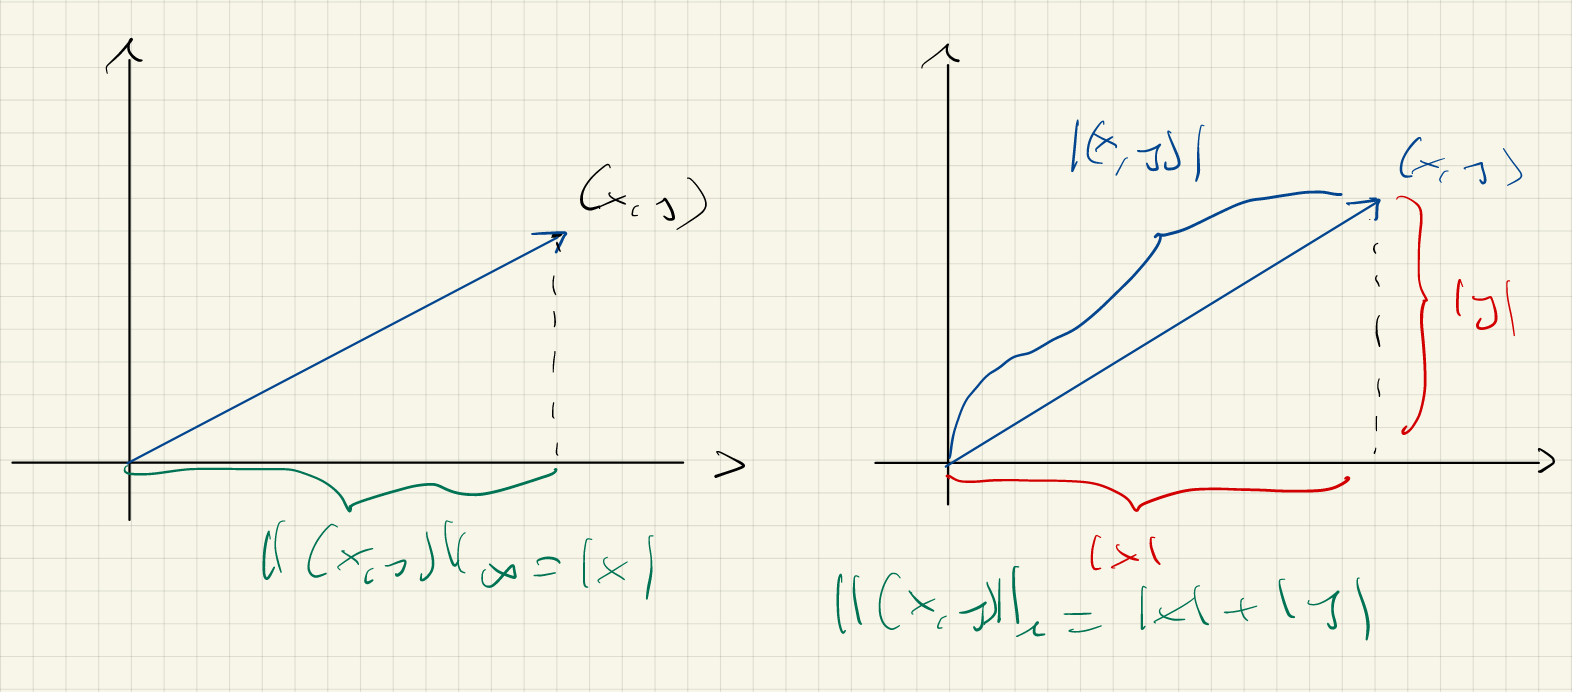
\includegraphics[width=\textwidth]{Screenshot from 2023-03-22 16-09-06.png}
\end{figure}
$\parallel\overline{x}\parallel_p = \left( \sum_{i=1}^{n}|x_i|^p \right)^{\frac{1}{p}},\,\,\, p \geq 1$\\
$\parallel\overline{x}\parallel_\infty = \lim_{p \rightarrow +\infty} \parallel\overline{x}\parallel_p$\\
$(\R^n,||\cdot||_p)$ è spazio normato

\begin{itemize}
	\item $C^\circ([0,1])$\\
	$\parallel f\parallel_\infty = \sup_{x \in [0,1]} |f(x)| \textcolor{orange}{(=\max_{x \in [0,1]} |f(x)|)}$\\
	$\parallel f\parallel_1=\int_{0}^{1} |f(x)|dx$\\
	$\parallel f\parallel_p= \left( \int_{0}^{1} |f(x)|^p dx\right)^{\frac{1}{p}}\,\,\,\, p \geq 1$\\
	sono tute norme su $C^\circ([0,1])$
\end{itemize}
Faccio vedere che $\parallel\cdot\parallel_\infty$ su $C^\circ([0,1])$ è una norma
\begin{enumerate}
	\item $\parallel f\parallel_\infty \geq 0$ (banale)\\
	$\parallel f\parallel_\infty =  0 \Leftrightarrow \sup_{x \in [0,1]}|f(x)|=0 \Leftrightarrow 0 \leq |f(x)| \leq0 \,\,\, \forall x \in[0,1] \Leftrightarrow f(x)=0\,\,\, \forall x\in[0,1]$
	\item $\parallel \lambda f\parallel_\infty = |\lambda|\parallel f\parallel_\infty \forall \lambda \in \R$ e $\forall f \in C^\circ([0,1])$\\
	$\parallel \lambda f\parallel_\infty = \sup_{x \in[0,1]}|\lambda f(x)|=\sup_{x\in[0,1]}|\lambda||f(x)|=|\lambda|\sup_{x\in[0,1]}|f(x)|=|\lambda|\parallel f\parallel_\infty$
	\item $\parallel f+g\parallel_\infty \leq \parallel f\parallel_\infty + \parallel g\parallel_\infty \,\,\, \forall f,g \in C^\circ([0,1])$\\
	$\parallel f+g\parallel_\infty = \sup_{x\in[0,1]} |f(x)+g(x)|$\\
	$|f(x)+g(x)| \leq |f(x)|+|g(x)|\leq \sup_{y\in[0,1]} |f(y)|+\sup_{y\in[0,1]} |g(y)|= \parallel f\parallel_\infty + \parallel g\parallel_\infty \,\,\, \forall x \in [0,1]$\\
	$\parallel f+g\parallel_\infty = \sup_{x\in[0,1]} |f(x)+g(x)|\leq \parallel f\parallel_\infty + \parallel g(x)\parallel_\infty$\\
\end{enumerate}
Facciamo vedere che $\parallel f\parallel_1 = \int_{0}^{1}|f(x)|dx$ è una norma
\begin{enumerate}
	\item $\parallel f \parallel_1 \geq 0\,\,\, \forall f\in C^\circ([0,1]) banale$\\
	Dimostriamo che $\parallel f \parallel_1=0 \Leftrightarrow f(x)=0\,\,\, \forall x\in[0,1]$\\
	$\Leftarrow) f(x)=0\,\,\, \forall x \in[0,1]$\\
	$\parallel f \parallel_1 =\int_{0}^{1}0dx=0$\\
	$\Rightarrow)$ Sia $\parallel f\parallel_1=0$ e dimostriamo che $f(x)=0\,\,\, \forall x \in [0,1]$\\
	$\int_{0}^{1}|f(x)|dx=0$\\
	Se $\exists x_0 \in [0,1]$ tale che $|f(x_0)|\neq 0$ allora $\exists$ un intorno $U$ di $x_0 $ tale che $|f(x)| \geq \frac{|f(x_0)|}{2}$ $\forall x \in U \cap [0,1]$ 
	\begin{itemize}
		\item $U=]x_0-\delta, x_0+\delta[ \subseteq [0,1]$
		\item $x_0=0$\\ $U=]0-\delta,0+\delta[$\\
		$U \cap [0,1]=[0,\delta[$
		\item $x_1=1$\\ $U=]1-\delta,1+\delta[$\\
		$U \cap [0,1]=]1-\delta,1]$
	\end{itemize}
	cioè in ogni caso $U \cap [0,1]$ è un intervallo di ampiezza almeno $\frac{\delta}{2}>0$\\
	$\parallel f\parallel_1=\int_{0}^{1} |f(x)|dx \geq \int_{U \cap [0,1]} |f(x)|dx \geq \int_{U\cap [0,1]} \frac{|f(x_0)|}{2}dx \geq \frac{\delta}{4}|f(x_0)|>0$\\
	il che è assurdo, perchè $\parallel f\parallel_1=0$
	\item $\parallel \lambda f\parallel_1=\int_{0}^{1}|\lambda f(x)|dx= |\lambda|\int_{0}^{1}|f(x)|dx = |\lambda|\parallel f\parallel_1\,\,\,\, \lambda\in \R$
	\item $f,g \in C^\circ([0,1])$\\
	$||f+g||_1=\int_{0}^{1}|f(x)+g(x)|dx \leq \int_{0}^{1}(|f(x)|+|g(x)|)dx = ||f||_1+||g||_1 \Rightarrow$ vale la disuguaglianza triangolare
\end{enumerate}
Dato uno spazio normato $(X,\parallel\cdot\parallel)$ posso definire la distanza tra due vettori $x,y \in X$ come $d(x,y)= \parallel x-y\parallel$, lunghezza del vettore $x-y$.

\begin{figure}[h!]
	\centering
	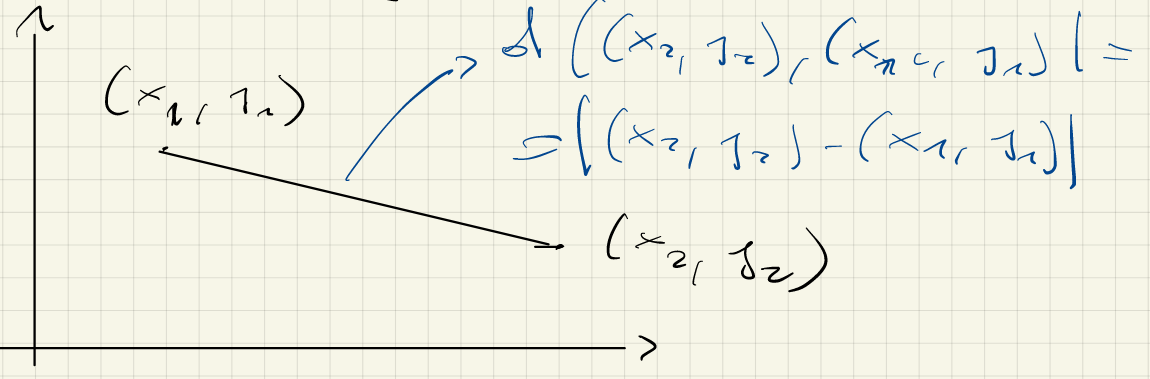
\includegraphics[width=\textwidth]{Screenshot from 2023-03-22 16-56-15.png}
\end{figure}

\paragraph{\textcolor{red}{Definizione}}
$X$ insieme non vuoto. Una distanza o metrica su $X$ è una funzione $d:X \times X\rightarrow \R$ tale che
\begin{enumerate}
	\item $d(x,y)\geq 0 \,\,\, \forall x,y \in X $ e $d(x,y)=0 \Leftrightarrow x=y$
	\item $d(x,y)=d(y,x)$ proprietà simmetrica
	\item Disuguaglianza triangolare $d(x,y)\leq d(x,z)+d(z,y) \,\,\, \forall x,y,z \in X$
\end{enumerate}
La coppia $(X,d)$ si dice \textcolor{red}{spazio metrico}.






	
	
\end{comment}